%%%%%%%%%%%%%%%%%%%%%%%%%%%%%%%%%%%%%%%%%
% Short Sectioned Assignment
% LaTeX Template
% Version 1.0 (5/5/12)
%
% This template has been downloaded from:
% http://www.LaTeXTemplates.com
%
% Original author:
% Frits Wenneker (http://www.howtotex.com)
%
% License:
% CC BY-NC-SA 3.0 (http://creativecommons.org/licenses/by-nc-sa/3.0/)
%
%%%%%%%%%%%%%%%%%%%%%%%%%%%%%%%%%%%%%%%%%

%----------------------------------------------------------------------------------------
%	PACKAGES AND OTHER DOCUMENT CONFIGURATIONS
%----------------------------------------------------------------------------------------

\documentclass[paper=a4,margin=0.5cm]{scrartcl} % A4 paper and 11pt font size

\usepackage{geometry}
\geometry{a4paper,left=2cm,right=2cm,top=1cm,bottom=1cm}




\usepackage{fourier} % Use the Adobe Utopia font for the document - comment this line to return to the LaTeX default
\usepackage[english]{babel} % English language/hyphenation
\usepackage{amsmath,amsfonts,amsthm} % Math packages

\usepackage{sectsty} % Allows customizing section commands
\allsectionsfont{\centering \normalfont\scshape} % Make all sections centered, the default font and small caps

%\usepackage{fancyhdr} % Custom headers and footers
%\pagestyle{fancyplain} % Makes all pages in the document conform to the custom headers and footers
%\fancyhead{} % No page header - if you want one, create it in the same way as the footers below
%\fancyfoot[L]{} % Empty left footer
%fancyfoot[C]{} % Empty center footer
%\fancyfoot[R]{\thepage} % Page numbering for right footer
%\renewcommand{\headrulewidth}{0pt} % Remove header underlines
%\renewcommand{\footrulewidth}{0pt} % Remove footer underlines
%\setlength{\headheight}{13.6pt} % Customize the height of the header


\usepackage[UTF8]{ctex}
\usepackage{url}
\usepackage{graphicx}
\usepackage{pythonhighlight}

\usepackage{indentfirst}
\setlength{\parindent}{2em}

%----------------------------------------------------------------------------------------
%	TITLE SECTION
%----------------------------------------------------------------------------------------

\newcommand{\horrule}[1]{\rule{\linewidth}{#1}} % Create horizontal rule command with 1 argument of height

\title{	
\normalfont \normalsize 
\textsc{University of Chinese Academy of Sciences} \\ [25pt] % Your university, school and/or department name(s)
\horrule{0.5pt} \\[0.4cm] % Thin top horizontal rule
\huge 计算机算法设计与分析 \\ % The assignment title
\horrule{2pt} \\[0.5cm] % Thick bottom horizontal rule
}

\author{李睿易} % Your name

\date{\normalsize\today} % Today's date or a custom date

\begin{document}

\maketitle % Print the title
\tableofcontents

%----------------------------------------------------------------------------------------
%	综述
%----------------------------------------------------------------------------------------
\section{综述}
\indent 实现了TSP,0/1背包问题,Las vegas算法,并对其性能进行分析,所有算法的单组数据运行时间控制在1000s以内,平均为600s。所有的代码均使用Python3,运行内存为16GB,CPU频率为2.6Ghz。\\
\indent 该作业的所有数据,代码和本文的Latex源码已经上传到github: \\
\indent \url{https://github.com/AresDemmo/Algorithm/tree/master/algorithm_design_and_analysis/DeadWork} \\
\indent 文件排列如下:\\
\begin{enumerate}
		\item Output:存放输出数据
		\item Package:存放三个0/1背包算法的源码
		\item TSP:存放三个TSP算法的源码
		\item EleTable:电路板布线问题算法的源码
		\item data:存放输入数据
		\item GenerateData.py:产生三个问题的输入数据
		\item work.tex:本文的latex源码
\end{enumerate}


%----------------------------------------------------------------------------------------
%	Program TSP
%----------------------------------------------------------------------------------------

\section{Program TSP}

\indent \textbf{问题:} 上机实现TSP的模拟退火算法,随机生成一定规模的数据或用通用数据集比较其它人的结果,分析算法的性能,摸索实现中技术问题的解决。\\
\indent \textbf{数据:} 随机生成一百组数据,城市数量为1到100,为每一条边随机赋值。\\
\indent \textbf{算法:} 实现了以下三种TSP算法并进行分析:\\
\indent (1)TSP-Force.py:暴力算法,n!的复杂度直接枚举解。\\
\indent (2)TSP-Search.py:分支限界搜索算法,按照当前代价最小的优先队列进行搜索。\\
\indent (3)TSP-SA.py:模拟退火算法。\\


\subsection{TSP暴力算法}

\indent 暴力算法,直接枚举城市的全排列,并对每一个结果进行比较得到最优解,主代码如下:\\
\begin{python}
def TSP_Force():
	path = [i for i in range(n)]
	cost = CalCulate_length(path)
	for i in itertools.permutations(path, n):#枚举序列
		c = CalCulate_length(i)
		if c < cost:
			cost = c
			path = copy.deepcopy(i)
	return (cost, path)
\end{python}

\indent 运行结果,在运行到城市数为10的时候就已经接近一分钟了,后面的数据处理为指数级增长。\\

\begin{tabular}{cccccccccc}
	\hline 
	数据量: & 2 & 3 & 4 &5 &6 &7 &8 &9 &10 \\ 
	\hline 
	运行时间:&0 &0 &0 &0 &0 &0 &0 &4 &49 \\ 
	\hline 
	运行结果:&37 &189 &72 &128 &161 &165 &90 &116 &122\\ 
	\hline 
\end{tabular} 



\subsection{TSP分支界限法}

\indent 分支界限算法,按照当前节点路径长度最小的优先级设置优先队列,对当前搜索到的节点,如果代价已经超过目前的最优值则剪枝。主代码如下:\\
\begin{python}
def TSP_Search():
	ans = Node(n * 1000, n, [])
	a = Node(0, 1, [0])
	que = PriorityQueue()
	que.put(Node(0, 1, [0]))
	while not que.empty():
		node = que.get()
		A = node.path[node.deep - 1]
		if node.deep == n:
			if node.cost + table[A][0] < ans.cost:#无法得到更优的解则剪枝
				ans.copy(node)
				ans.cost = node.cost + table[A][0]
			continue
		for i in range(n):
			if not i in node.path:
				cost = node.cost + table[A][i]
				if cost < ans.cost:
					que.put(Node(cost, node.deep + 1, node.path + [i]))
	return (ans.cost, ans.path)
\end{python}

\indent 运行结果,在小规模的数据中性能要优于暴力算法,但是当城市数大于15时,搜索性能较差,结果如下:\\

\begin{tabular}{ccccccccccccccc}
	\hline 
	数据量: & 2 & 3 & 4 & 5 & 6 & 7 & 8 & 9 & 10 & 11 & 12 & 13 & 14 & 15\\ 
	\hline 
	运行时间:& 0 & 0 & 0 & 0 & 0 & 0 & 0 & 0 & 1 & 4 & 11 & 33 & 148 & 439 \\ 
	\hline 
	运行结果:& 37 & 189 & 72 & 128 & 161 & 165 & 90 & 116 & 122 & 145 & 154 & 179 & 176 & 157\\ 
	\hline 
\end{tabular}



\subsection{TSP模拟退火算法}
\indent 模拟退火算法,设置参数:Speed=0.9,Temp=1000,L=10,主代码如下:\\
\begin{python}
def TSP_SA():
	r, t, t_min = Speed, Initial_Temp, 0.001
	p = [i for i in range(n)]
	cost = CalCulate_length(p)
	temp, bestone = Node(cost, p), Node(cost, p)
	while t > t_min:
		for i in range(L):
			getNewSolution(temp)
			temp.length = CalCulate_length(temp.path)
			if (Accept(bestone, temp, t)):
				bestone.copy(temp.length, temp.path)
			else:
				temp.copy(bestone.length, bestone.path)
		t *= r
	return (bestone.length, bestone.path)
\end{python}

\indent 运行结果,首先,对比前十五组数据准确度以及时间效率(同搜索算法进行比较),结果如下:\\
\begin{tabular}{ccccccccccccccc}
	\hline 
	数据量: & 2 & 3 & 4 & 5 & 6 & 7 & 8 & 9 & 10 & 11 & 12 & 13 & 14 & 15\\ 
	\hline 
	运行时间占比:& 3.0 & 3.0 & 5.0 & 6.0 & 8.0 & 10.0 & 12.0 & 15.0 & 17.0 & 5.0 & 2.0 & 0.78 & 0.19 & 0.07 \\ 
	\hline 
	结果准确度:& 1.0 & 1.0 & 1.0 & 1.0 & 1.0 & 1.0 & 1.0 & 1.0 & 1.28 & 1.0 & 1.18 & 1.08 & 1.09 & 1.28\\ 
	\hline 
\end{tabular}
\\
\indent 通过以上表格可以看出,小数据量上模拟退火算法并没有时间优势,但是数据规模越大,在保持较高精度的同时运行时间更少,图1是模拟退火算法在100以内的数量级上的运行时间图。\\
\begin{figure}
	\centering
	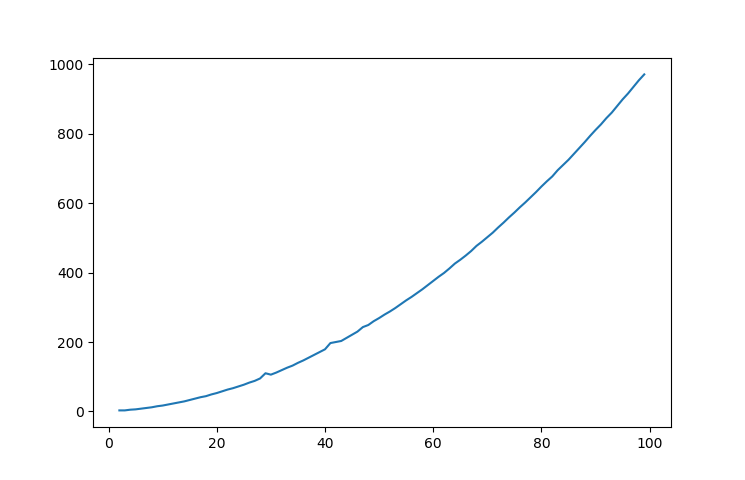
\includegraphics[width=0.7\linewidth]{TSPSA}
	\caption{TSP-SA运行时间图}
	\label{fig:tspsa}
\end{figure}




%----------------------------------------------------------------------------------------
%	Program 0/1背包
%----------------------------------------------------------------------------------------


\section{Program 0/1背包}


\indent \textbf{问题:} 上机实现0/1背包问题的遗传算法。\\
\indent \textbf{数据:} 随机生成一百组数据,物品数量为100-10000,每一百个为界,随机生成物品重量和占用空间,均为1-10的整数。\\
\indent \textbf{算法:} 实现了以下三种0/1背包算法并进行分析,每一种算法都可以在10000个物品的规模中在1000s左右生成解:\\
\indent (1)Package-Force.py:暴力算法,枚举序偶。\\
\indent (2)Package-Search.py:分支限界搜索算法,按照当前LU函数值进行搜索。\\
\indent (3)Package-SA.py:遗传算法。\\

\subsection{Package暴力算法}

\indent 暴力算法,实现讲义中的枚举序偶的算法,主代码如下:\\
\begin{python}
def Package_Force(A, C):
	cnt = [[0,0]]
	value = 0
	for i in range(len(A)):
		cns = []
		for j in range(len(cnt)):
			if (A[i][0] + cnt[j][0] <= C):
				cns += [[A[i][0] + cnt[j][0], A[i][1] + cnt[j][1]]]
				value = max(value, A[i][1] + cnt[j][1])
		cnt = Merge(cnt, cns)
return value
\end{python}

\indent 运行结果,处理时间基本呈线性增长,但是在一些特殊的数据中会表现的较差,主要是数据无法有效减少序偶的个数,因此时间相对来说会相对变长,以下是部分数据的运行结果:\\
\begin{tabular}{cccccccccccccc}
	\hline 
	数据量: & 0 & 800 & 1600 & 2400 & 3200 & 4000 & 4800 & 5600 & 6400 & 7200 & 8000 & 8800 & 9600\\ 
	\hline 
	运行时间:& 0 & 6 & 24 & 74 & 135 & 192 & 279 & 310 & 241 & 310 & 891 & 461 & 552 \\ 
	\hline 
	运行结果:& 0 & 2893 & 5927 & 12211 & 16326 & 17997 & 21716 & 20517 & 16387 & 18283 & 43697 & 22063 & 24594\\ 
	\hline 
\end{tabular}


\subsection{Package分支界限法}

\indent 分支界限算法,按照讲义中的分支限界法进行实现。主代码如下:\\
\begin{python}
def DKpackage(P, W, N, M, e):
	global tables
	tables = []
	(pvl, pvu) = LUBound(P, W, M, 0, N, 1)
	node = getNode(0, 0, 0, M, 0, pvu)
	prev = pvl - e
	que = PriorityQueue()
	que.put(node)
	while not que.empty():
		node = que.get()
		i = node.level + 1
		cap = node.CC
		cv = node.CV
		if node.CUB <= prev:
			break
		if i == N + 1:
			if cv > prev:
				prev = cv
				answer = node
		else:
			if cap >= W[i]:
				cntnode = getNode(node.id, i, 1, cap - W[i], cv + P[i], node.CUB)
				que.put(cntnode)
			(pvl, pvu) = LUBound(P, W, cap, cv, N, i + 1)   
			if pvu > prev:
				cntnode = getNode(node.id, i, 0, cap, cv, pvl)  
				que.put(cntnode)
	return answer
\end{python}

\indent 运行结果,在各种数据集中的表现结果都优于序偶暴力算法,可以在得到最优解的情况下大幅度减少运行时间:\\
\begin{tabular}{cccccccccccccc}
	\hline 
	数据量:& 0 & 800 & 1600 & 2400 & 3200 & 4000 & 4800 & 5600 & 6400 & 7200 & 8000 & 8800 & 9600\\ 
	\hline 
	运行时间:& 0 & 1 & 4 & 2 & 3 & 6 & 10 & 69 & 27 & 22 & 20 & 45 & 60 \\ 
	\hline 
	运行结果:& 0 & 2893 & 5927 & 12211 & 16326 & 17997 & 21716 & 20517 & 16387 & 18283 & 43697 & 22063 & 24594\\ 
	\hline 
\end{tabular}


\subsection{Package遗传算法}
\indent 遗传算法,在进行算法实现的时候,随机过程很容易得不到一个解,于是陷入无限随机过程,在算法中加入随机因子,按照物品总重占背包空间的大小来随机解,并且按照千分之三的概率进行变异。在随机解的过程中,如果当前解超过背包,加大从1到0的变异概率。主代码如下:\\
\begin{python}
def Package_GA():
	global newpop, oldpop
	if (n == 0):
		return 0
	initpop()
	statistics(newpop)
	gen = 0 
	while(gen < maxgen):
		gen = gen + 1
		oldmax = maxfitness
		oldmaxpop = maxpop
		generation()
		statistics(newpop)
		if (maxfitness < oldmax):
			newpop[minpop] = copy.deepcopy(oldpop[oldmaxpop])
			statistics(newpop)
		#直接换引用,加快速度
		t = oldpop
		oldpop = newpop
		newpop = t
return maxfitness
\end{python}

\indent 运行结果,轮盘赌的方式产生结果较差,在迭代求解过程中很难找到一个较优的解,主要算法时间耗费在生成一个可行解上,时间效率接近序偶暴力算法,但是仅能达到50\%的最优值,结果如下:\\
\begin{tabular}{ccccccccccccccc}
	\hline 
	数据量: & 800 & 1600 & 2400 & 3200 & 4000 & 4800 & 5600 & 6400 & 7200 & 8000 & 8800 & 9600\\ 
	\hline 
	运行时间:& 43 & 81 & 115 & 152 & 190 & 232 & 275 & 374 & 411 & 379 & 497 & 535 \\ 
	\hline 
	运行结果:& 1702 & 3399 & 7187 & 9378 & 11525 & 13585 & 10989 & 6812 & 7609 & 23025 & 8988 & 10067\\ 
	\hline 
\end{tabular}


%----------------------------------------------------------------------------------------
%	Program 电路板布线
%----------------------------------------------------------------------------------------

\section{Program 电路板布线}
\indent \textbf{问题:}上机实现Las vegas算法结合分枝限界算法解决电路板布线问题,分析算法性能。\\
\indent \textbf{数据:} 随机生成20组数据,每一组数据为1000*1000的表格,通过宽度优先搜索确保每一组数据都有解,并且不同组数据中的障碍物逐渐降低,从50\%到5\%依次下降。\\
\indent \textbf{算法:} Las Vegas算法与分支界限算法相结合的方法,算法如下:当前队列中存在超过40个节点的时候,进行五次Las Vegas算法降低节点数量,主代码如下:\\

\begin{python}
def LasVagas():
	cnt = numpy.zeros((n, m))
	que = PriorityQueue()
	que.put(Node(startx, starty, 0))
	cnt[startx][starty] = 1
	isLas = 0
	NodeNum = 0
	value = -1
	while not que.empty():
		node = que.get()
		NodeNum += 1
		if (node.x == endx and node.y == endy):
			value = node.deep
			break
		k = random.randint(0, 3)
		if isLas == 0 and que.qsize() > 40:
			isLas = LasStart
		for i in range(4):
			if isLas > 0 and i != k:
				continue            
			nx = node.x + dx[i]
			ny = node.y + dy[i]
			if (nx < 0 or nx >= n or ny < 0 or ny >= m):
				continue
			if (cnt[nx][ny] == 0 and table[nx][ny] != '1'):
				cnt[nx][ny] = node.deep + 1
				que.put(Node(nx, ny, node.deep + 1))
		if isLas > 0:
			isLas -= 1
		return (NodeNum, value)
\end{python}

\indent 运行结果,在1000*1000的表格中,障碍物大量存在,如果终点位于一个相对封闭的位置(即周围存在大量障碍物),随机过程很难找到结果。随机选择的过程中,很容易将可以得到解的路径随机掉,而且由于排除掉了这些可能得到结果的路径后,搜索节点会大量上升。每一组数据随机运行了100次LasVegas算法并于搜索过程进行对比:\\
\begin{tabular}{ccccccccccccccccccccc}
	
	\hline 
	数据组数:&1 &2 &3 &4 &5 &6 &7 &8 &9 &10 &11 &12 &13 &14 &15 &16 &17 &18 &19 &20\\
	\hline 
	LasVegas运行时间: & 14 & 14 & 20 & 13 & 9 & 8 & 7 & 10 & 9 & 5 & 9 & 8 & 8 & 9 & 8 & 9 & 9 & 8 & 8 & 8\\ 
	\hline 
	Search运行时间:& 44 & 16 & 69 & 19 & 19 & 45 & 16 & 79 & 80 & 1 & 35 & 61 & 23 & 84 & 27 & 90 & 63 & 4 & 28 & 16 \\ 
	\hline 
	LasVegas搜索节点数(w):& 14 & 15 & 20 & 16 & 17 & 17 & 15 & 20 & 19 & 11 & 19 & 17 & 16 & 19 & 16 & 19 & 19 & 17 & 16 & 17\\ 
	\hline 
	Search搜索节点数(w):& 54 & 19 & 83 & 24 & 22 & 54 & 19 & 83 & 92 & 1 & 41 & 64 & 23 & 79 & 27 & 78 & 64 & 4 & 28 & 17\\ 
	\hline 
	运行时间占比:& 0.34 & 0.92 & 0.30 & 0.70 & 0.47 & 0.19& 0.47 & 0.13 & 0.12 & 5.86 & 0.274 & 0.13 & 0.35 & 0.11 & 0.31 & 0.10 & 0.15 & 2.23 & 0.29 & 0.54\\ 
	\hline 
	搜索节点数占比:& 0.25 & 0.78 & 0.24 & 0.66 & 0.77& 0.31 & 0.78 & 0.24 & 0.20 & 11.0 & 0.46 & 0.26 & 0.69 & 0.24 & 0.59 & 0.24 & 0.29 & 4.25 & 0.57 & 1.0\\ 
	\hline 
	运行成功率:& 25 & 41 & 14 & 26 & 17 & 23 & 21 & 15 & 15 & 47 & 16 & 25 & 14 & 22 & 21 & 15 & 19 & 21 & 14 & 23\\ 
	\hline 
\end{tabular}

\indent 通过以上数据可以看出,以上随机决策在数据是随机的状况下,随机过程找到解的概率并不会因障碍物减少就增加,反而是对起点终点位置很敏感。如果起点或者终点位于障碍物较多的地方,即便障碍物仅仅只占空间的5\%,但是找到解的概率并不会因此上升。\\
\indent 我们可以看到第三组数据,只有14\%的成功率,但是时间占比和搜索占比都比较小,说明该组数据在随机的过程中很容易失去最优解。而在第十组数据中,随机过程更容易把搜索方向导向更差的路径上去,因此虽然成功率高,但是时间运行效率都比搜索要慢很多。\\
\indent 不同的随机决策都会有不同的问题,在减少搜索数量和快速得到解中间需要权衡,而且不同的随机决策在起点和终点位于障碍物较多的地方的数据上表现就远远达不到预期。\\


\end{document}